\documentclass[11pt]{article} % use larger type; default would be 10pt

\usepackage[utf8]{inputenc} % set input encoding (not needed with XeLaTeX)

\usepackage{geometry} % to change the page dimensions
\geometry{a4paper} % or letterpaper (US) or a5paper or....

\usepackage{graphicx} % support the \includegraphics command and options

%%% PACKAGES
\usepackage{amssymb}
\usepackage{amsmath}
\usepackage{booktabs} % for much better looking tables
\usepackage{array} % for better arrays (eg matrices) in maths
\usepackage{paralist} % very flexible & customisable lists (eg. enumerate/itemize, etc.)
\usepackage{verbatim} % adds environment for commenting out blocks of text & for better verbatim
\usepackage{subfig} % make it possible to include more than one captioned figure/table in a single float
\usepackage{listings} % used to write pieces of code
\usepackage{xcolor}
\usepackage{hyperref} % used to generate external links
% These packages are all incorporated in the memoir class to one degree or another...

%%% HEADERS & FOOTERS
\usepackage{fancyhdr} % This should be set AFTER setting up the page geometry
\pagestyle{fancy} % options: empty , plain , fancy
\renewcommand{\headrulewidth}{0pt} % customise the layout...
\newcommand{\code}{\texttt}
\lhead{}\chead{}\rhead{}
\lfoot{}\cfoot{\thepage}\rfoot{}

%%% SECTION TITLE APPEARANCE
\usepackage{sectsty}
\allsectionsfont{\sffamily\mdseries\upshape} % (See the fntguide.pdf for font help)
% (This matches ConTeXt defaults)

%%% ToC (table of contents) APPEARANCE
\usepackage[nottoc,notlof,notlot]{tocbibind} % Put the bibliography in the ToC
\usepackage[titles,subfigure]{tocloft} % Alter the style of the Table of Contents
\renewcommand{\cftsecfont}{\rmfamily\mdseries\upshape}
\renewcommand{\cftsecpagefont}{\rmfamily\mdseries\upshape} % No bold!
\newcommand{\qed}{\hfill $\blacksquare$}
%%% END Article customizations

%%% The "real" document content comes below...

\title{FOR project (prof. Federico Malucelli)}
\author{Corigliano Emilio - 10627041 - 995098}
\date{A.A. 2021/22} % Activate to display a given date or no date (if empty)

\begin{document}
\maketitle

\section{Introduction}
We are given a set of houses with parcticular positions that, with a cost, can become minimarkets if they gave the permission. All the minimarkets, then, have to be refurbished by a truck. Every truck has a maximum of minimarkets they can supply (capacity), a fixed cost and a cost for every km travelled on the path. The objective is to minimize the cost of both the construction and the refurbishment.

The solution has been made creating a python script and dividing the problem in two main subproblems, the opening of the minimarkets and their refurbishment.

\section{Solution}
The solution is composed of three main steps:
\begin{itemize}
\item Optimal solution of the construction of the minimarkets
\item Search for the best grouping of minimarkets with a greedy algorithm
\item Optimal hamiltonian cycle for each route
\end{itemize}

\subsection{Opening of the minimarkets}
The solution is an optimal solution of the first part done with a python framework for solving linear programming problems called \textit{ortools}. So, after modeling the first part of the problem (as previously done for the miniproject), the framework solves it and minimizes the construction cost in the optimal way.

\subsection{Search for the best routes}
The markets are grouped in order to minimize the amount of routes and to minimize their distance. In order to do that, the points are ordered in base of the angle of the line that connect the point one to the others [\ref{fig:angle ordering}]. For this reason, the groups are taken so that the angular displacement of all the group is minimal (ordering the points in base of their "angle" and then splitting this ordered array in different contiguous subarrays). This process is done several times with different starting nodes and different maximum capacities in order to find the best grouping of the nodes. To evaluate the goodness of each grouping a greedy algorithm has been used: it starts from the central facility and searches the closest point of that group, once selected we search for the closest point from the last added one and so on. 
\begin{figure}[h]
    \centering
    \subfloat[\centering]{{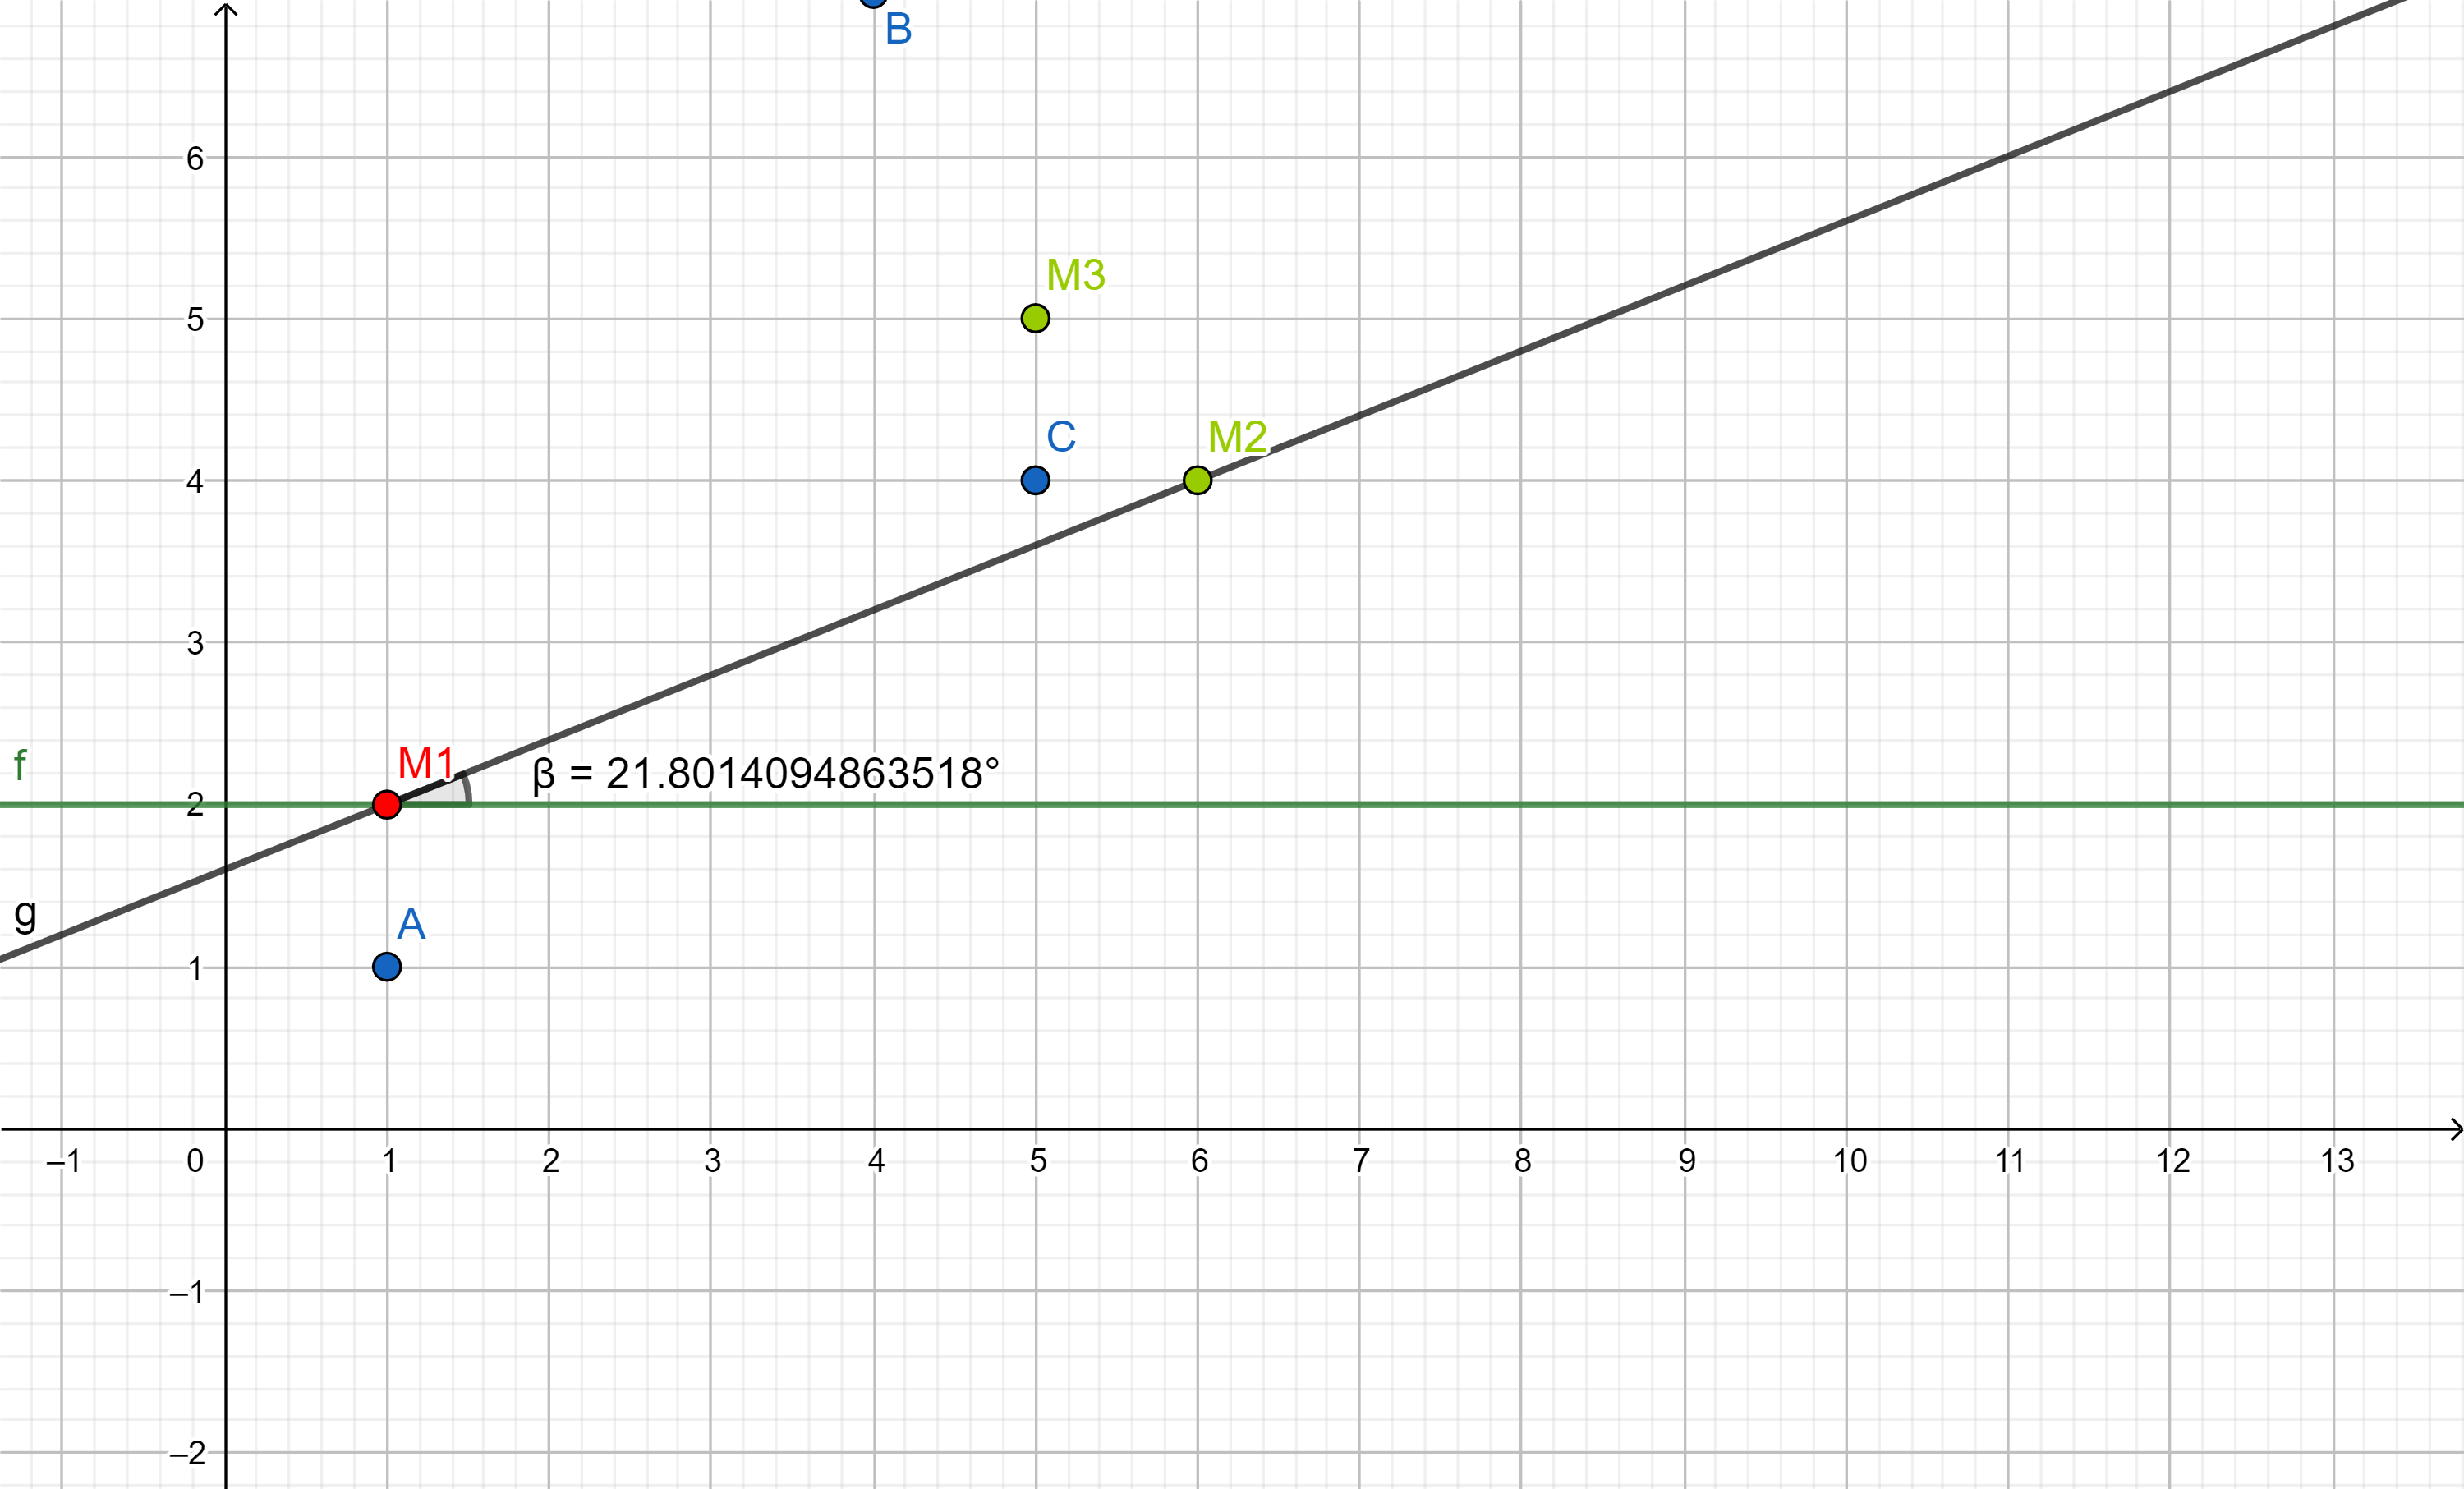
\includegraphics[width=0.40\textwidth]{angle1.png} }}%
    \qquad
    \subfloat[\centering]{{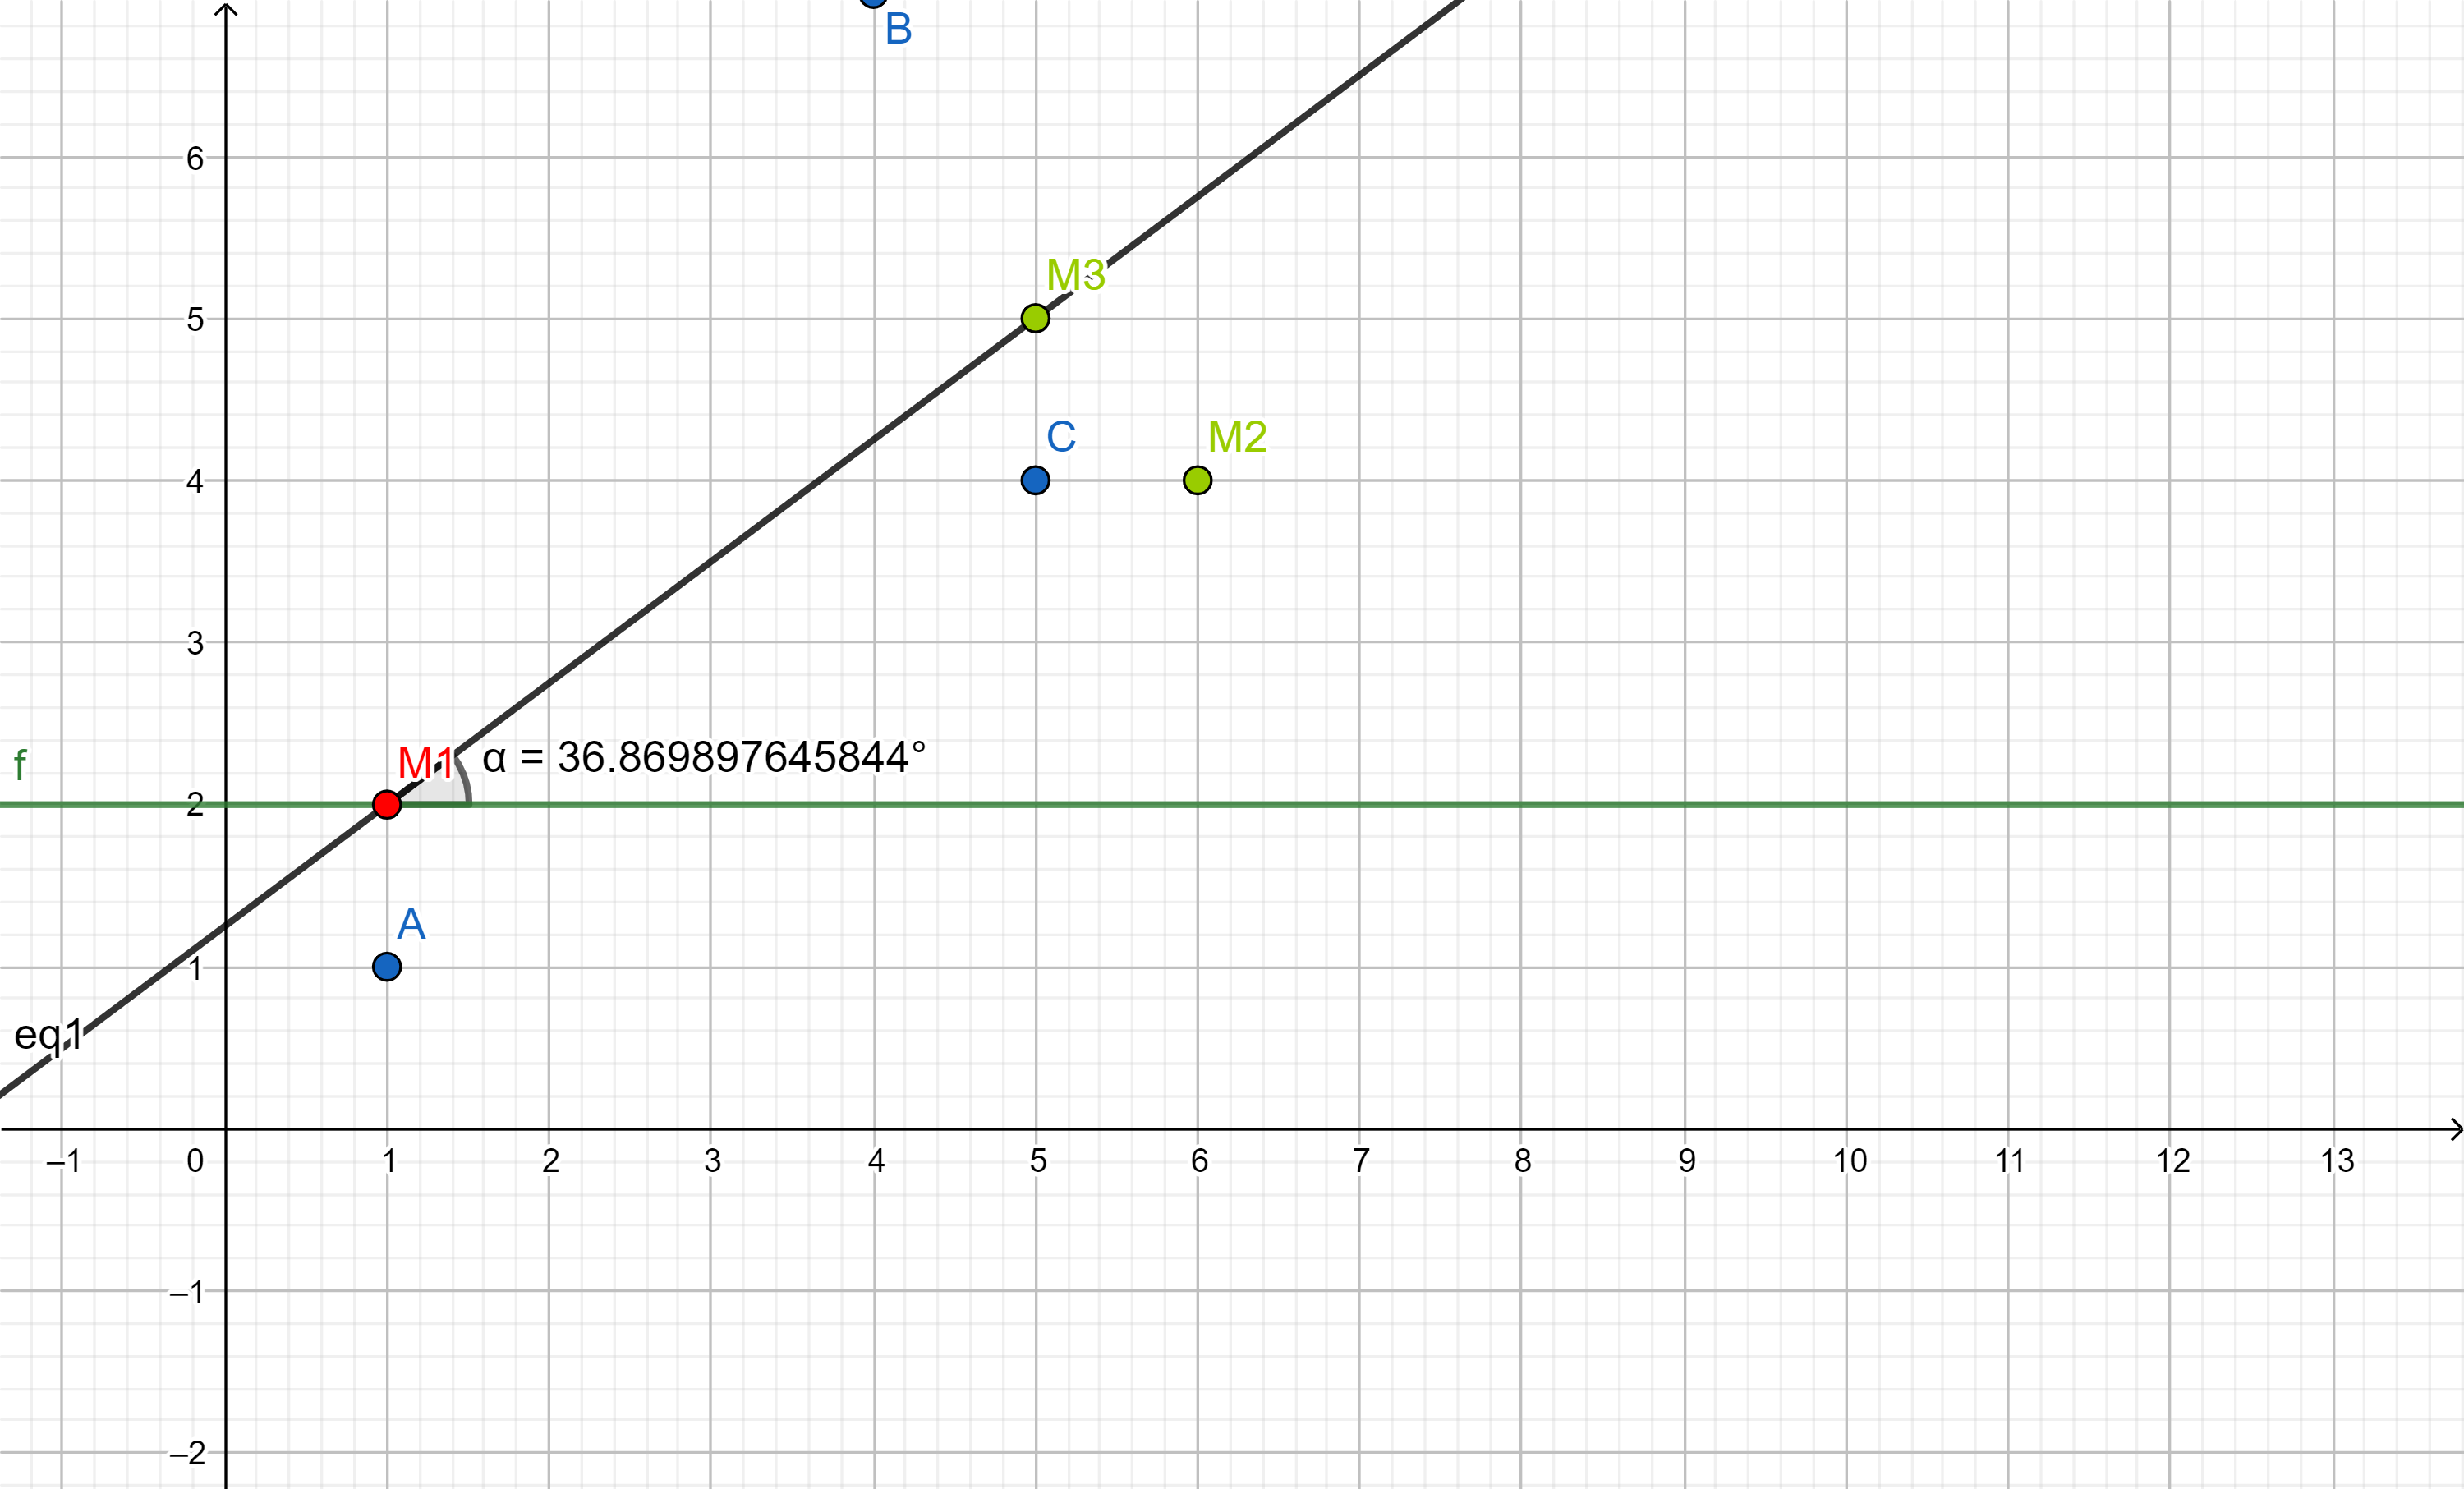
\includegraphics[width=0.40\textwidth]{angle2.png} }}%
    \caption{In this case M2 is "lesser" than M3, so it will be chosen before M3}%
    \label{fig:angle ordering}%
\end{figure}

\subsection{Path of the routes}
After selecting the most promising grouping, if the group is small enough not to exceed the time constraint, we use an exact (but optimized) solver for the minimum hamiltonian cycle. It checks for every possible route the cost and stores the best one. This problem is represented by the worst case of the TSP problem, when the graph is fully connected, for this reason an exact fast algorithm doesn't exist at the moment (because it's an NP-complete problem). Anyway in this problem half of the combinations can be discarded because are just a reflection of a considered one (so the execution time is sharply an half). The script dynamically checks if we can proceed with the exact method or if we are running out of time (and so, we must use the greedy version of the algorithm)

\section{Results}
The best solution found is stored in a txt file. In addition, a png graph is generated for each solution considered in roder to to see a visual solution of the problem [\ref{fig:optimal graphs}]; in here the grey points are the houses, the green points are the minimarkets and the red point is the central facility. Using this method, setting a high enough time limit, the solutions found are:
\begin{itemize}
\item minimart-I-50: Total=344.657, Opening=65, Refurbishment=279.657
\item minimart-I-100: Total=887.684, Opening=166, Refurbishment=721.684
\end{itemize}

\begin{figure}[h]
    \centering
    \subfloat[\centering minimart-I-50]{{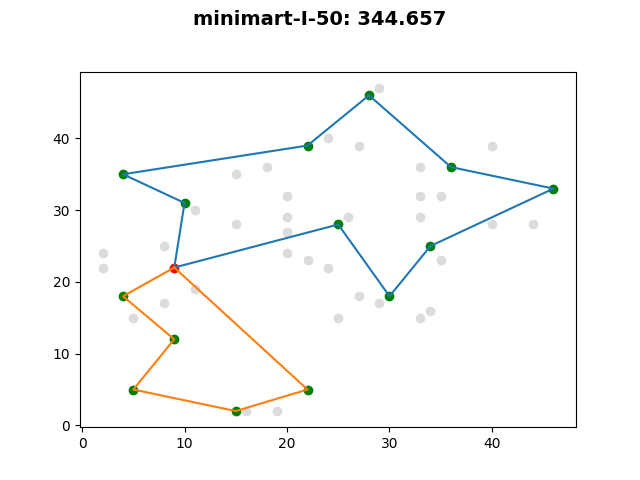
\includegraphics[width=0.45\textwidth]{../minimart-I-50-optimal.png} }}%
    \qquad
    \subfloat[\centering minimart-I-100]{{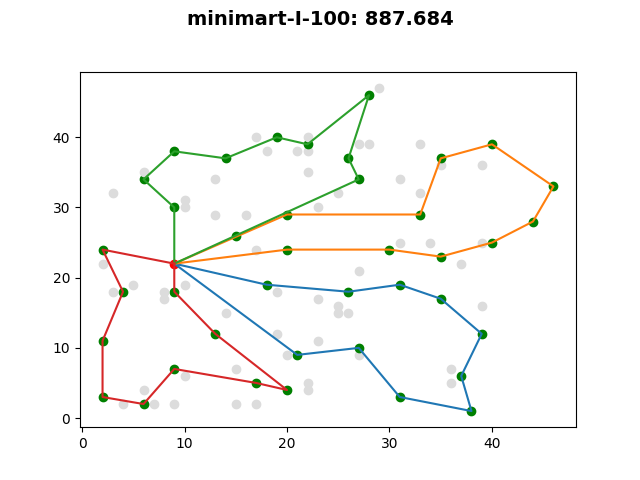
\includegraphics[width=0.45\textwidth]{../minimart-I-100-optimal.png} }}%
    \caption{Solutions of the proposed cases}%
    \label{fig:optimal graphs}%
\end{figure}

\section{Possible upgrades}
Maybe it could be implemented a better approximation of the minimum hamiltonian cycle finder, checking if the arcs intersect or not and trying to get a non intersecting cycle with more advanced methods.
\end{document}